\chapter{Results}\label{cha:Research}
%

% Ska följa som ett naturligt komplement till huvuddelen

In this chapter, the results are presented, so that in the next chapter, these results are analysed.

%\section{Example}\label{sec:research:history}
%
Liksom \citep{Duck:2005} har vi kommit fram till att glass smakar bäst på sommaren \citep{Khalil02NonlinearSystemsBook}.

\marginpar{Kommer att tänka på en liten anekdot\ldots}

\Warning[TODO]{Ta bort den löjliga anekdoten!}

\begin{figure}[tbp]
  \centering
  \subfloat[Alldeles för tidigt.][\label{fig:times:very-early}Det här är väl tidigt — din glass hinner smälta innan ditt sällskap dyker upp.]{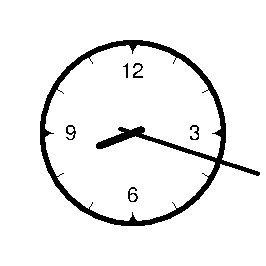
\includegraphics[page=1]{clocks}}
  \qquad
  \subfloat[Med marginal.][\label{fig:times:early}Kiosken stänger snart, men inte nu — perfekt!]{\includegraphics[page=2]{clocks}}
  \\
  \subfloat[I grevens tid.][\label{fig:times:on-time}Precis i tid — du får in ett finger i luckan just när kiosken ska stänga.  Han som jobbar blir sur, och det blir smolk i bägaren.]{\includegraphics[page=3]{clocks}}
  \qquad
  \subfloat[Försent.][\label{fig:times:late}Du är sen — kiosken är stängd.]{\includegraphics[page=4]{clocks}}
  \caption{\label{fig:times}%
    Illustration av \emph{subfloats}.  Den så kallade \emph{bounding box}en visas i \protect\subref{fig:times:late}.  Lägg märke till att bounding boxen har satts så att alla bilder har samma storlek, med enhetlig placering av själva innehållet i förhållande till bounding boxen.  Antag att du ska träffa en kompis för att äta glass just när kiosken stänger för dagen vid 08:30.  När dyker du upp?}
\end{figure}

\section{Developed Application}

  Here the results from the app for iteration 2, 3 and 4 are shown. Iteration 1 is missing, as the app development had not started.

  \subsection{Iteration \#1}

  There was no developed application at this point.

  Instead, two workshops were held, which together would inform the future development of an application.

  There were the findings from those two workshops:

  \subsubsection{Workshop \#1: Customer Journey Map: A day as a coach}

  \subsubsection{Workshop \#2: Quizical and Duolingo}


  \subsection{Iteration \#2}

  \subsubsection{Result}
  Quiz-flödet 1.0: standard multiple-choice, designat för assessment, men ej för learning
  Besvara multiple-choice-frågor
  Få resultat-tavla med Question 1: 0, Question 2: 1, samt "Total score: X/X"
  Gå tillbaka till startskärm

  \subsection{Iteration 3}

  \subsubsection{Result}

  Quiz flow 2.0 was designed for learning and self-reflection

  \begin{itemize}
  \item vid varje fråga besvarar du det alternativ du tror är rätt samt "Are you sure?" Yes/No
  \item vid färdigt quiz, få en resultattavla med personliserad feedback
  \item läsa igenom dina felaktiga svar och hur säker du varit på dem
  \item observerat de korrekta svaren
  \item klicka "Improve" för att bara få dina felaktiga svar igen
  upprepa tills inga felaktiga svar var kvar (det står "quiz try: 3", om det är försök 3)
  \item vid 100%, låsa upp "I can get 100%" (som är hela quizet igen)
  \item innan dess, uppmuntrades du läsa igenom coach/deltagar-manualen
  \item om du då fick något fel, fick du gå tillbaka till träning igen
  \item om alla rätt på, blev du Certified coach. Om du klarade det på första försöket, fick du även en guldstjärna (andra försöket = silver, tredje försöket = brons)
  \item sedan kunde du ta ett annat quiz
  \end{itemize}

  Kommentar, fördelar med feedback-läge:
  Genom att på varje fråga besvara "Are you sure?": Yes/No, så stärker vi inte bara coachens meta-kognitiva förmåga, utan vi kan vi även ge personliserad feedback i resultattavlan, istället för att bara visa Question 1: 1 point. Question 2: 0 points, som i Iteration 2.

  Detta gör att coachen kan reflektera över sitt lärande på t.ex. följande sätt:
  - få en självförtroende-boost (via feedback "You were correct, and you were sure")
  - gå från gissning till självsäkerhet (via feedback "You guessed, but you were correct")
  - ändra uppfattning snabbare (via feedback "You were incorrect, but you were sure")
  - uppmuntra coachen att läsa i manualen (via feedback "You were incorrect, and you were not sure")

  Fördelar med tränings-läge, och certifikations-läge:
  From Josefina: "Jag gillar idén att när coachen har kunnat svara rätt på alla frågor, kunna befästa kunskapen med hjälp av certifikations-läget, då coachen ska kunna få 100\% rätt på 1 försök."

  \subsection{Iteration \#4}

  %Result

  \todo{Show images of final app - on mobile, tablet and desktop?}


\section{Qualitative Data}

  Here the results from the qualitative data for iteration 1, 2, 3 and 4 are shown.

  \subsection{Qualitative data}

\subsubsection{Entrepreneurship education considerations}
Throught early interviews with YoungDrive staff, it is clear that YoungDrive's entrepreneurship education methodology goes hand in hand with the presented theory. It's mottos are: "Dream big, start small", "Learning by doing" and "We have fun!" \citep{youngdrive}.

Both in regards to designing for the users and for the above reason, the app should be a complement to YoundDrive's existing training material and the structure of the program.

A challenging part of the work is that YoungDrive consists of both the practical skills of the entrepreneur, theoretical material of running a business, and an entrepreneurial mindset. Therefore, both how to assess knowledge, and build habits, needs to be examined.

\subsubsection{Understanding the coach situation}

A CBT can be responsible for from 7 up to 12 different youth groups in different programs, and such a high number places huge demands on the CBT.

Even if there are only 7 groups, being behind on schedule or not being confident, can be very demanding.

\textbf{Stayover at Patrick:} På morgonen visade Patrick mig hur han jobbar med deras tomt, var det odlas ris, och andra råvaror, deras djur, deras story från Syd-Sudan, till Kampala, till hyddan här i Tororo, och hans värderingar.

Efter en ungdomssession nästföljande dag besökte vi och hälsade kort på en av de 2 CBT:s vi har session med idag. Sedan hade jag och Patrick den obligatoriska review av ungdoms-sessionen, och jag bjöd honom på middag. Kl. 19 ringde hans fru (som har börjat få tecken av malaria) och skyndade hem.

Nästa ungdomssession fick jag besöka en annan CBT. Vi var tidiga. Sedan började jag prata med henne, och fick bra tillfälle att intervjua henne och även förklara för henne vad jag gjorde där. Det blev underligt att förklara för henne: Patrick påminde, när jag tabbat mig, att “Marcus, du måste förklara för X vad en app är”. Så hon fick låna min mobil, och jag förklarade att app var kort för applikation, och att för varje applikation har ett eget syfte, t.ex. ta foton. Jag bad henne klicka, svårt, råkade klicka åt henne, men sedan lät jag henne göra. Efter hon sett att det hon såg i skärmen var det hon såg på riktigt, blev hon jätteglad och började fundera vad hon skulle fota. Hon reste sig och gick runt hörnet, och jag följde efter. Hon fotade, efter att noggrannt tänkt igenom, att hon fotade buskarna med frukt. Sedan sade jag hon kunde fortsätta fota, och då tog hon ett litet runt hus utanför.


\subsubsection{Different kind of coaches}

The interviews with CBTs, PLs and stakeholders led to the realization that different coaches handles this differently well.

Depending on the situation, e.g. you are not confident, or you are falling behind with the schedule, you can be in one of these need groups.

\begin{itemize}
  \item The ideal coach
  \item The realistic coach
  \item The challenged coach
\end{itemize}

It was discovered, that coach confidence comes largely from being able to have good youth sessions.

\subsubsection{A good youth session}

For having a good youth session, these are the most important attributes:

\begin{itemize}
  \item Correct information
  \item Correct structure
  \item Time management
  \item Fun atmosphere
\end{itemize}

The fact that the coach knows they have these qualities, leads to self confidence from the coach. This in turn, leads to better meetings with the youth.

\subsubsection{The room for a digital solution}

It is definitely a problem that so extremely few have smartphones.

This needs to be designed for. Either, I build only for the use case of having an app tailored for the coach training, where the donated devices can be used.

Alternatively, I design only for the users that does have a smartphone, and count that more will get smartphones in the future.

Thirdly, I can use a SMS tool, not building an app but an SMS-based service, which also could be an app. Such tools exists, and are compatible with multiple-choice questions, like VOTO Mobile.

  \subsection{Qualitative data}

\subsubsection{Design workshop \#1 in Zambia}

The result was fantastic, in the sense that it gave me an unbiased look at what the coaches expected from the app, what functionality wasn't important, and into their technical preferences.

The designs and insights gained were used throughout the week to further improve the app I had actually started creating, and gave great insights to who the coaches were and their thinking. \todo{Add image here}

\subsubsection{The desire perspective}

Insight: "The app could be used on my spare time". This is particularly true, about the bonus quizzes that were produced during the week.

Insight: \textit{Coach:} "I'll buy one" (a smartphone), \textit{Response from other coaches: } "Whoa!"

\subsubsection{The utility perspective}

Ideation: "The app should have notes, not only quesitions"

\subsubsection{The usability perspective}

Low resolution screens, made the text be barely visible. This showed, that the app needed to be tested on a lot of different devices. This is particularly true, as on day 1, the coaches did not know how to zoom, which could cause accident refreshs, frustration or confusion.

The app needs to work offline! To be online on the phone is too expensive for the coaches, and too unrealiable to give a satisfactory experience. Also, during testing, relying on internet can cause a lot of problems, especially if the teacher is alone.

\subsubsection{The learning perspective}

    The coaches had surprisingly high results, and at day 3 they wished harder questions when asked.

    We responded by having harder questions, e.g. by introducing similar answers, and testing 4 alternatives instead of 3. This was appreciated.

    The following analysis could be done:

    \subsubsection{Doing a pre-quiz: good for learning}
    When asked about what they thought about doing "Graduation" as a pre-quiz (before the session), 10/10 said they liked doing the quiz before, and that it benefited their learning during the session.

    When asked why it helped, these were the results:

    \begin{itemize}
    \item "During session, it is easier to follow" - 10 (100\%)
    \item "Giving the paper manuals before, scanning headings and pictures etc, would not help" - 10 (100\%)
    \end{itemize}

    It was also tested to work in group or individually. The ones who answered, said that you learned more individually (3/3), and more fun doing it together (3/3). Doing it together, was enjoyable as it was "Very easy because of using different minds" and "We can collaborate to do better".

    \subsubsection{Doing a post-quiz: Spaced versus massed learning}
    In "Goal setting", quotes were "I thought it was fun and challenging to do the quiz immediately afterwards", with another coach commenting "The mind was still fresh".

    When asked on timing preference, 10/10 said it would be more fun to do the quiz immediately afterwards, not at the end of the day. The motivation, seemed to be that it was easier.

    9/10, said they wanted to do the quiz afterwards. The outlier, said it would be better for learning doing it later.

    After this comment, this was the distribution:

    \begin{itemize}
    \item 3/10 wants to do the quiz both before and after a session
    \item 1/10 wants to do the quiz before and at the end of the day
    \item 7/10 wants to do the quiz only immediately afterwards
    \item 10/10 wants to do the quiz immediately afterwards, and then again at the end of the day
    \item 7/10 wants to do the quiz immediately afterwards, and then a joined quiz with other topics at the end of the day
    \end{itemize}

\subsubsection{The teacher perspective}

  \textbf{Low scores}
  The 9/19 shows the relevancy of the quiz, as Josefina did not think she would have discovered that the coach was lagging behind otherwise.

  In the data, it was observable that the coach had done well together with others, but 3/7 when done individually.

  Josefina said about the 9/19: "This is where a control group would be beneficial". "He is often passive during open questions, but active during the team exercises."

  The question we needed to ask ourselves, was: "Does this imply he is a good or bad coach?".

  \textbf{What would hinder Josefina from using the app}

  Josefina says: "Not doing data collection digitally works whenever they are 10 - but not with bigger numbers than that."

  According to the final interview with Josefina, she does not wish the app to replace her. She enjoys teaching, thinks she has an important role, and suggests the app to be designed to support her and the coaches, not replace her.

  \textbf{Acceptance criteria}

  If you have a high score, you are ready. If not, you need to redo the quiz.

  If you are 8/10 or lower, you are in the red zone. If lower than 10/10, they are not ready, the motivation being that what they don't know, they will teach in an improper way: affecting hundreds of youth. This is why Josefina thinks they should need all of the answers correct.

  \textbf{Testing Correct Structure, Time Management and Fun Atmosphere}
  Josefina informs that Correct Structure, Time Management and Fun Atmosphere would be the most valuable to test after a youth session. She also notes, that \textit{some} aseessment could be made via the app before a session. Because of the reason that this thesis does not focus on after-session-evaluation, Correct Information is primary to improving on the other factors, which are secondary.

\subsubsection{The developer perspective}

  \begin{itemize}
    \item Bugs was a big hindrance to functionality, and a lot (both high-dose, and high-scale) of testing is very important
    \item Simpler design than I thought (KISS) was sufficient
  \end{itemize}

\subsubsection{Bonus results: Testing the app on Kampala university student}
The app was tested on a university student from Makarere University.

The university student from Makarere University scored 100\% correct, in spite of not having any entrepreneurship training. This showed that guessing was possible, or that the quizzes were too easy.

  \subsection{Qualitative data}

  %What the observations said

  \subsubsection{Observations from Kampala test}
  The entrepreneurship student in Kampala, informed the following changes:

  Instead of "Become certified", he would be more motivated by unlocking the opportunity to apply the skills.

  "Improve" should be renamed "Try again", because it is more intuitive.

  His overall opinion on the app was:

  "Can you give me the link, because I'd love to do more of this. I think it's amazing."

  \subsubsection{Verified relevancy of seperating Training and Certification}
  When asked for an opinion, Josefina answered: "I like the idea that when the coaches have answered all of the questions correctly, they can consilidate the knowledge by the certification test, when the coach should get 100\% correct on their first try."

  \subsubsection{Field visits}

  The first thought was to use Gold/Silver/Bronze in the Training mode, and "Are you sure?" in the Certification mode. User tests showed that the other way around was better.

  \subsubsection{Big app test}
  \textbf{Learning: } The app test simulated the app being used to assess preparedness for a youth session. They clearly showed evidence between the difference between designing for Assessment and Learning:

  Given a coach having prepared for their youth session on week 9, and then only scoring 5/10, what should happen? In a similar way, what should happen if 9/10 correct answers?

  For the coach training, the assessment was okay, since Josefina could pick up and give feedback.

  Before a youth session, leaving the coach there is not viable. If the coach has 9/10, that coach should not only be let be, and especially if the score has been 5/10.

  Feedback was that one user did not want to press "Improve", until having read the manual. The motivation was: "Not because that is what the info says, but because I can learn more from the manual, about more than what the questions says."

  This is indeed the preferred behaviour from Josefina, and the app should continue to encourage only using the app training or certification mode after having prepared via the manual. This way, the app is still assessment, but it is "learning by thinking", with feedback.

  \subsection{Iteration \#4}

Everyone now thought the app was good and easy to use.

With the Plan Tororo staff, it was shown how important the certification mode was: even though one group had 100\% on their first try, and a person had 1 wrong answer, the person with 1 wrong answer got 100\% on the certification, while the 100\% group had 1 wrong answer.

It is therefore determined, that when all of the answers can be answered correctly, after having gotten all answers correct once, that the knowledge is reliable - this is deliberate practice.


\section{Quantitative Data}

  Here the results from the quantitative data for iteration 1, 2, 3 and 4 are shown.

  \subsection{Qualitative data}

\subsubsection{Entrepreneurship education considerations}
Throught early interviews with YoungDrive staff, it is clear that YoungDrive's entrepreneurship education methodology goes hand in hand with the presented theory. It's mottos are: "Dream big, start small", "Learning by doing" and "We have fun!" \citep{youngdrive}.

Both in regards to designing for the users and for the above reason, the app should be a complement to YoundDrive's existing training material and the structure of the program.

A challenging part of the work is that YoungDrive consists of both the practical skills of the entrepreneur, theoretical material of running a business, and an entrepreneurial mindset. Therefore, both how to assess knowledge, and build habits, needs to be examined.

\subsubsection{Understanding the coach situation}

A CBT can be responsible for from 7 up to 12 different youth groups in different programs, and such a high number places huge demands on the CBT.

Even if there are only 7 groups, being behind on schedule or not being confident, can be very demanding.

\textbf{Stayover at Patrick:} På morgonen visade Patrick mig hur han jobbar med deras tomt, var det odlas ris, och andra råvaror, deras djur, deras story från Syd-Sudan, till Kampala, till hyddan här i Tororo, och hans värderingar.

Efter en ungdomssession nästföljande dag besökte vi och hälsade kort på en av de 2 CBT:s vi har session med idag. Sedan hade jag och Patrick den obligatoriska review av ungdoms-sessionen, och jag bjöd honom på middag. Kl. 19 ringde hans fru (som har börjat få tecken av malaria) och skyndade hem.

Nästa ungdomssession fick jag besöka en annan CBT. Vi var tidiga. Sedan började jag prata med henne, och fick bra tillfälle att intervjua henne och även förklara för henne vad jag gjorde där. Det blev underligt att förklara för henne: Patrick påminde, när jag tabbat mig, att “Marcus, du måste förklara för X vad en app är”. Så hon fick låna min mobil, och jag förklarade att app var kort för applikation, och att för varje applikation har ett eget syfte, t.ex. ta foton. Jag bad henne klicka, svårt, råkade klicka åt henne, men sedan lät jag henne göra. Efter hon sett att det hon såg i skärmen var det hon såg på riktigt, blev hon jätteglad och började fundera vad hon skulle fota. Hon reste sig och gick runt hörnet, och jag följde efter. Hon fotade, efter att noggrannt tänkt igenom, att hon fotade buskarna med frukt. Sedan sade jag hon kunde fortsätta fota, och då tog hon ett litet runt hus utanför.


\subsubsection{Different kind of coaches}

The interviews with CBTs, PLs and stakeholders led to the realization that different coaches handles this differently well.

Depending on the situation, e.g. you are not confident, or you are falling behind with the schedule, you can be in one of these need groups.

\begin{itemize}
  \item The ideal coach
  \item The realistic coach
  \item The challenged coach
\end{itemize}

It was discovered, that coach confidence comes largely from being able to have good youth sessions.

\subsubsection{A good youth session}

For having a good youth session, these are the most important attributes:

\begin{itemize}
  \item Correct information
  \item Correct structure
  \item Time management
  \item Fun atmosphere
\end{itemize}

The fact that the coach knows they have these qualities, leads to self confidence from the coach. This in turn, leads to better meetings with the youth.

\subsubsection{The room for a digital solution}

It is definitely a problem that so extremely few have smartphones.

This needs to be designed for. Either, I build only for the use case of having an app tailored for the coach training, where the donated devices can be used.

Alternatively, I design only for the users that does have a smartphone, and count that more will get smartphones in the future.

Thirdly, I can use a SMS tool, not building an app but an SMS-based service, which also could be an app. Such tools exists, and are compatible with multiple-choice questions, like VOTO Mobile.

  \subsection{Qualitative data}

\subsubsection{Design workshop \#1 in Zambia}

The result was fantastic, in the sense that it gave me an unbiased look at what the coaches expected from the app, what functionality wasn't important, and into their technical preferences.

The designs and insights gained were used throughout the week to further improve the app I had actually started creating, and gave great insights to who the coaches were and their thinking. \todo{Add image here}

\subsubsection{The desire perspective}

Insight: "The app could be used on my spare time". This is particularly true, about the bonus quizzes that were produced during the week.

Insight: \textit{Coach:} "I'll buy one" (a smartphone), \textit{Response from other coaches: } "Whoa!"

\subsubsection{The utility perspective}

Ideation: "The app should have notes, not only quesitions"

\subsubsection{The usability perspective}

Low resolution screens, made the text be barely visible. This showed, that the app needed to be tested on a lot of different devices. This is particularly true, as on day 1, the coaches did not know how to zoom, which could cause accident refreshs, frustration or confusion.

The app needs to work offline! To be online on the phone is too expensive for the coaches, and too unrealiable to give a satisfactory experience. Also, during testing, relying on internet can cause a lot of problems, especially if the teacher is alone.

\subsubsection{The learning perspective}

    The coaches had surprisingly high results, and at day 3 they wished harder questions when asked.

    We responded by having harder questions, e.g. by introducing similar answers, and testing 4 alternatives instead of 3. This was appreciated.

    The following analysis could be done:

    \subsubsection{Doing a pre-quiz: good for learning}
    When asked about what they thought about doing "Graduation" as a pre-quiz (before the session), 10/10 said they liked doing the quiz before, and that it benefited their learning during the session.

    When asked why it helped, these were the results:

    \begin{itemize}
    \item "During session, it is easier to follow" - 10 (100\%)
    \item "Giving the paper manuals before, scanning headings and pictures etc, would not help" - 10 (100\%)
    \end{itemize}

    It was also tested to work in group or individually. The ones who answered, said that you learned more individually (3/3), and more fun doing it together (3/3). Doing it together, was enjoyable as it was "Very easy because of using different minds" and "We can collaborate to do better".

    \subsubsection{Doing a post-quiz: Spaced versus massed learning}
    In "Goal setting", quotes were "I thought it was fun and challenging to do the quiz immediately afterwards", with another coach commenting "The mind was still fresh".

    When asked on timing preference, 10/10 said it would be more fun to do the quiz immediately afterwards, not at the end of the day. The motivation, seemed to be that it was easier.

    9/10, said they wanted to do the quiz afterwards. The outlier, said it would be better for learning doing it later.

    After this comment, this was the distribution:

    \begin{itemize}
    \item 3/10 wants to do the quiz both before and after a session
    \item 1/10 wants to do the quiz before and at the end of the day
    \item 7/10 wants to do the quiz only immediately afterwards
    \item 10/10 wants to do the quiz immediately afterwards, and then again at the end of the day
    \item 7/10 wants to do the quiz immediately afterwards, and then a joined quiz with other topics at the end of the day
    \end{itemize}

\subsubsection{The teacher perspective}

  \textbf{Low scores}
  The 9/19 shows the relevancy of the quiz, as Josefina did not think she would have discovered that the coach was lagging behind otherwise.

  In the data, it was observable that the coach had done well together with others, but 3/7 when done individually.

  Josefina said about the 9/19: "This is where a control group would be beneficial". "He is often passive during open questions, but active during the team exercises."

  The question we needed to ask ourselves, was: "Does this imply he is a good or bad coach?".

  \textbf{What would hinder Josefina from using the app}

  Josefina says: "Not doing data collection digitally works whenever they are 10 - but not with bigger numbers than that."

  According to the final interview with Josefina, she does not wish the app to replace her. She enjoys teaching, thinks she has an important role, and suggests the app to be designed to support her and the coaches, not replace her.

  \textbf{Acceptance criteria}

  If you have a high score, you are ready. If not, you need to redo the quiz.

  If you are 8/10 or lower, you are in the red zone. If lower than 10/10, they are not ready, the motivation being that what they don't know, they will teach in an improper way: affecting hundreds of youth. This is why Josefina thinks they should need all of the answers correct.

  \textbf{Testing Correct Structure, Time Management and Fun Atmosphere}
  Josefina informs that Correct Structure, Time Management and Fun Atmosphere would be the most valuable to test after a youth session. She also notes, that \textit{some} aseessment could be made via the app before a session. Because of the reason that this thesis does not focus on after-session-evaluation, Correct Information is primary to improving on the other factors, which are secondary.

\subsubsection{The developer perspective}

  \begin{itemize}
    \item Bugs was a big hindrance to functionality, and a lot (both high-dose, and high-scale) of testing is very important
    \item Simpler design than I thought (KISS) was sufficient
  \end{itemize}

\subsubsection{Bonus results: Testing the app on Kampala university student}
The app was tested on a university student from Makarere University.

The university student from Makarere University scored 100\% correct, in spite of not having any entrepreneurship training. This showed that guessing was possible, or that the quizzes were too easy.

  \subsection{Qualitative data}

  %What the observations said

  \subsubsection{Observations from Kampala test}
  The entrepreneurship student in Kampala, informed the following changes:

  Instead of "Become certified", he would be more motivated by unlocking the opportunity to apply the skills.

  "Improve" should be renamed "Try again", because it is more intuitive.

  His overall opinion on the app was:

  "Can you give me the link, because I'd love to do more of this. I think it's amazing."

  \subsubsection{Verified relevancy of seperating Training and Certification}
  When asked for an opinion, Josefina answered: "I like the idea that when the coaches have answered all of the questions correctly, they can consilidate the knowledge by the certification test, when the coach should get 100\% correct on their first try."

  \subsubsection{Field visits}

  The first thought was to use Gold/Silver/Bronze in the Training mode, and "Are you sure?" in the Certification mode. User tests showed that the other way around was better.

  \subsubsection{Big app test}
  \textbf{Learning: } The app test simulated the app being used to assess preparedness for a youth session. They clearly showed evidence between the difference between designing for Assessment and Learning:

  Given a coach having prepared for their youth session on week 9, and then only scoring 5/10, what should happen? In a similar way, what should happen if 9/10 correct answers?

  For the coach training, the assessment was okay, since Josefina could pick up and give feedback.

  Before a youth session, leaving the coach there is not viable. If the coach has 9/10, that coach should not only be let be, and especially if the score has been 5/10.

  Feedback was that one user did not want to press "Improve", until having read the manual. The motivation was: "Not because that is what the info says, but because I can learn more from the manual, about more than what the questions says."

  This is indeed the preferred behaviour from Josefina, and the app should continue to encourage only using the app training or certification mode after having prepared via the manual. This way, the app is still assessment, but it is "learning by thinking", with feedback.

  \subsection{Iteration \#4}

Everyone now thought the app was good and easy to use.

With the Plan Tororo staff, it was shown how important the certification mode was: even though one group had 100\% on their first try, and a person had 1 wrong answer, the person with 1 wrong answer got 100\% on the certification, while the 100\% group had 1 wrong answer.

It is therefore determined, that when all of the answers can be answered correctly, after having gotten all answers correct once, that the knowledge is reliable - this is deliberate practice.


\section{Insights}

  \subsection{Iteration \#1}

\subsubsection{Motivation of app}
The scope of the app is to examine and strengthen the entrepreneurship the student already has. One important goal is to give good feedback.

The users are already motivated. Thus, I can follow Sierra's advise designing for the compelling context.

My compelling context is that I want to help you become an even better coach.

The better user point of view: don’t just make a better coach training app - make a better user of coach training material.

For me, this means:

"Given a teaching situation among the youth group, a great coach can teach an entrepreneurship topic more consistent with what the coach material said."

"Given a question in the app, a great coach will get the right answer more often, and increasingly leverage the correct answer to their coach situation."

\subsubsection{Entrepreneurship education considerations}
The YoungDrive's entrepreneurship education methodology goes hand in hand with the presented theory. It's mottos are: "Dream big, start small", "Learning by doing" and "We have fun!" \cite{youngdrive}.

Both in regards to designing for the users and for the above reason, the app should be a complement to YoundDrive's existing training material and the structure of the program.

A challenging part of the work is that YoungDrive consists of both the practical skills of the entrepreneur, theoretical material of running a business, and an entrepreneurial mindset. Therefore, both how to assess knowledge, and build habits, needs to be examined.

  \subsection{Iteration \#2}

\subsubsection{Insights}

The app works for assessment!

  Using the quiz before the session increases learning, slightly decreases fun of the session, according to coaches

  Fun and encouraging

  \begin{itemize}
    \item The app works for assessment!
    \item Good for learning for the coaches
    \item A good indicator for Josefina
    \item A great way to scale the YoungDrive training in the future, both for online coach-training and the physical training
  \end{itemize}

After the meeting with the partner and expert group, the following was concluded from iteration \#2:

\begin{itemize}
\item The app is only working on assessment now, not for learning
\item The need for a field app still feels relevant (especially for sessions long since the coach training)
\item The potential for YoungDrive having online coach training is huge
\end{itemize}

Determine:
\begin{itemize}
  \item Focus for the next iteration: design quiz app for learning, focus on field app (CI, CS, TM, FA), and design having an app that works stand-alone from the YD coach training in mind.
\end{itemize}

Discussing the importance of self-reflection after a youth session with Josefina, led to asking more of such questions in coach quizzes.

Josefina: “I have a problem: there is no way I can control them how they have prepared themselves for a youth session."

An app could be used, either before you start planning (to guide what you need to study the most on), or after you think you are ready (so you can assess and improve).

\subsubsection{Bonus results: Testing the app outside the YoungDrive context}
Back in Uganda, a test was done with refugee innovators, at the Humanitarian Innovation Jam.

Also, the app was tested on a university student from Makarere University

The test with the refugee innovatiors were surprisingly intriguing and successful.

It was found that refugee innovators says they would have a great need for such an app.

The university student from Makarere University scored 100\% correct, in spite of not having any entrepreneurship training. This showed that guessing was possible, or that the quizzes were too easy.

\subsubsection{Findings}

Test with university student scored 100\% correct, means that common sense can go a long way, and that the results can't be 100\% trustworthy, and that multiple-choice questions has serious issues - this, we already knew during and before the coach training - but it needs to be taken care of

The app would be great and could actually work outside the physical coach training - with revision, be stand-alone, even being able to distribute online.

Now there are observable evidence for what the interactions from Iteration 1 showed:

\begin{itemize}
\item The purpose of the coach training should be to prepare the coach in having great youth sessions
\item Therefore, this is what the quizzess should assess
\item What it really means being a good YoungDrive coach, is having good youth sessions
\item Josefina would have liked to be able to stop coaches from having taught, if they do not have 90-100 \% correct information on the subject
\item Today, Josefina can not assess this. This means that some coaches, are teaching incorrect information to hundreds of youth.
\item Here, the quiz has a very good need to fill.
\end{itemize}

With all of these findings in summary, it can be concluded that an app for coach training, and an app to use before a youth session, could be the same app, since the purpose of preparing the coach to be great with its youth session is the same.

From the interviews, it was learned that while it \textit{may} be technically possible, the teacher desires the app support her, not replace her.

  \subsection{Iteration \#3}

  The app works for assessment!

  \begin{itemize}
    \item The app works for assessment!
    \item Good for learning for the coaches
    \item A good indicator for Josefina
    \item A great way to scale the YoungDrive training in the future, both for online coach-training and the physical training
  \end{itemize}

  \subsection{Iteration \#4}




%\begin{chapter-appendix}

%\section{Proof-Appendix}
%
Det här är en appendix-del av det aktuella kapitlet.

%\end{chapter-appendix}
